\documentclass[11pt]{article}
%%%%%%%%%%%%%%%%%%%%%%%%%%%%%%%%%%%%%%%%
\usepackage{amsmath}
\usepackage{verbatim}
\usepackage[usenames,dvipsnames]{color}
\usepackage{setspace}
\usepackage{lscape}
\usepackage{longtable}
\usepackage[top=1.25in,bottom=1.25in,left=1in,right=1in]{geometry}
\usepackage{graphicx}
\usepackage{epstopdf}
\usepackage[usenames,dvipsnames]{pstricks}
\usepackage{epsfig}
\usepackage{pstricks-add}
\usepackage{pst-node}
\usepackage{pst-plot}
\usepackage{fancyhdr}
\usepackage[absolute,showboxes]{textpos}
\usepackage{booktabs}
\usepackage{dcolumn}
\usepackage{arydshln}
\usepackage{natbib}
\usepackage{tabularx}
\usepackage{subfigure}
\usepackage{caption}
\usepackage{minitoc}
\usepackage{longtable}

\renewcommand{\thetable}{A.\arabic{table}}
\renewcommand{\thesection}{A.\arabic{section}}
\renewcommand{\theequation}{A.\arabic{equation}}
\makeatletter
\renewcommand{\l@section}{\@dottedtocline{1}{1.5em}{2.6em}}
\renewcommand{\l@subsection}{\@dottedtocline{2}{4.0em}{3.6em}}
\renewcommand{\l@subsubsection}{\@dottedtocline{3}{7.4em}{4.5em}}
\makeatother

\newtheorem{proposition}{Proposition}
\newtheorem{corollary}{Corollary}

\setcounter{MaxMatrixCols}{10}
\newcolumntype{d}[1]{D{.}{.}{-2.#1}}
\newenvironment{proof}[1][Proof]{\noindent\textbf{#1.} }{\ \rule{0.5em}{0.5em}}
\setlength{\columnsep}{.2in}
\psset{unit=1cm}

\def\sym#1{\ifmmode^{#1}\else\(^{#1}\)\fi}

\begin{document}
\begin{titlepage}
\hfill \textsc{FOR ONLINE PUBLICATION}

\vspace{1in} \noindent {\large \today}

\vspace{.5in} \noindent {\Large \textbf{\strut The role of land in temperate and tropical agriculture}}

\vspace{.25in} \noindent {\large T. Ryan Johnson}

\vspace{.05in} \noindent Washington University

\vspace{.25in} \noindent {\large Dietrich Vollrath}

\vspace{.05in} \noindent University of Houston

\vspace{2in} \noindent \textsc{Online Appendix} \hrulefill

\vspace{.05in} \noindent Robustness checks and alternative assumptions for empirical work from the main paper are contained here. Also included are definitions of countries included in regions used in paper, as well as additional theoretical work related to the model.
\vspace{.1in} \hrule

\end{titlepage}

\pagebreak 

\tableofcontents

\section{General version of empirical setup}
This is to demonstrate that the elasticity of agricultural productivity with respect to the density of agricultural labor is equal to the elasticity of agricultural output with respect to land given any constant returns to scale production function. Let agricultural production be
\begin{equation}
    Y_{Ai} = A_{Ai} F(X_i,K_{Ai},L_{Ai}) 
\end{equation}
for district $i$ in province $I$, where $F()$ is a constant returns to scale function with respect to the three inputs: land, capital, and labor. As in the main paper, we make the same mobility assumptions for labor and capital across districts, which again implies that $K_{Ai}/L_{Ai}$ is identical for all districts. 

Dividing the production function through by $L_{Ai}$ we have that
\begin{equation}
   Y_{Ai}/L_{Ai} = A_{Ai} F(X_i/L_{Ai},K_{Ai}/L_{Ai},1).
\end{equation}
Define $x_i = X_i/L_{Ai}$ and $k_{Ai} = K_{Ai}/L_{Ai}$ as the per-worker amounts of land and capital, and define
\begin{equation}
    f(x_i,k_{Ai}) = F(X_i/L_{Ai},K_{Ai}/L_{Ai},1)
\end{equation}
as the intensive form of the aggregate production function. By the mobility assumption, we know that $\phi_L Y_i/L_{Ai} = w$, where $\phi_L$ is the elasticity with respect to labor, and the wage is common across districts. This allows us to write that 
\begin{equation}
    w = \phi_L A_{Ai} f(x_i,k_{Ai}).
\end{equation}

Holding this wage constant as it is given by state-level factors, and noting that $k_{Ai}$ is also given by state-level factors, use the implicit function theorem to solve for
\begin{equation}
    \frac{\partial A_{Ai}}{\partial x_i} \frac{x_i}{A_{Ai}} = - \frac{\phi_L A_{Ai} f_1(x_i,k_{Ai})}{\phi_L f(x_i,k_{Ai})}\frac{x_i}{A_{Ai}} = - \frac{f_1(x_i,k_{Ai}) x_i}{f(x_i,k_{Ai})}.
\end{equation}
The elasticity of productivity, $A_i$, with respect to land per worker, $x_i$, is equal to the elasticity of $f()$ with respect to land per worker. This simply implies that the relationship of land per worker to productivity depends on how sensitive output per worker is to land per worker. 

It is straightforward to show, given the constant returns to scale production function, that
\begin{equation}
    \frac{f_1(x_i,k_{Ai}) x_i}{f(x_i,k_{Ai})} = \frac{F_1(X_i,K_{Ai},L_{Ai}) X_i}{F(X_i,K_{Ai},L_{Ai})}
\end{equation}
or that the elasticity of the intensive production function with respect to land per worker is equal to the elasticity of the aggregate production function with respect to land. Thus it follows that 
\begin{equation}
    \frac{\partial A_{Ai}}{\partial x_i} \frac{x_i}{A_{Ai}} = - \frac{F_1(X_i,K_{Ai},L_{Ai}) X_i}{F(X_i,K_{Ai},L_{Ai})}
\end{equation}
or that the elasticity of productivity with respect to land per worker, $x_i$, is equal to the negative of the elasticity of aggregate output with respect to land. It is then trivial that the elasticity of productivity with respect to density, $1/x_i$, is equal to the elasticity of aggregate output with respect to land. The Cobb-Douglas assumption used in the main paper is not necessary to derive the main estimating equation used in the paper.

\section{Specification with capital immobile between sectors}
In our main derivation, we assume that capital can move freely between agriculture and non-agriculture. If that were not true, then equation (8) in the main paper would be
\begin{equation}
    w_{As} = (1-\phi)(1-\beta) (1+\tau_{As}) p_{As} A_{Ais} \left(\frac{X_{is}}{L_{Ais}}\right)^{\beta} \left(\frac{K_{Ais}}{L_{Ais}}\right)^{\phi(1-\beta)},
\end{equation}
and our estimation would be based on
\begin{equation}
    \ln A_{Ais} = \beta \ln L_{Ais}/X_{is} - \phi(1-\beta) \ln K_{Ais}/L_{Ais} - \ln w_{As}/p_{As} - \ln (1+\tau_{As}) + \ln (1-\phi)(1-\beta).
\end{equation}
Here it becomes obvious that we need to control for \textit{agricultural capital per worker}, rather than aggregate capital per worker. The controls we use - nighttime lights, urban share, and total population - may not be as useful in controlling for this. However, in the robustness checks using DHS data on assets, we do have controls that are explicitly measuring rural assets (livestock, etc..). As these results conform to our baseline, it does not appear that this assumption about mobile capital is driving our results. 

\section{Explicit two-sector model}\label{APP_solve}
In Section 2 of the paper we derived our estimation equation for $\beta$, and this was done using an aggregate agricultural production function, but without reference to any specific preferences. Here we add assumptions regarding preferences and non-agricultural production so that we can solve for the agricultural labor share and real income per capita in a state as a whole. We show that the elasticity $\beta$ influences how sensitive real income and the share of labor in agriculture are to population and technological change. That model shows that as $\beta$ gets \textit{higher}, the economy gets \textit{more} sensitive to population and technological change.

\subsection{State-level agricultural and non-agricultural production}
The agricultural sector operates as described in Section 2 of the main paper. We also continue with the assumptions made in the main paper, namely that $p_{Ais} = p_{As}$, $w_{Ais} = w_{Nis} = w_{s}$, and $r_{Ais} = r_{Nis}$. To that we add the assumption that $r_{Ais} = r_{Nis} = r_{s}$, or that capital is mobile across districts within a state. 

These assumptions imply that $K_{Ais}/L_{Ais} = K_{Nis}/L_{Nis} = K_{is}/L_{is} = K_s/L_s$, or that the capital output ratio in each sector, in each district, is identical. This can be seen by examining equations (4) and (7) in the main paper, which show the capital output ratio of a sector in a district as proportion to the wage/rental ratio, which is identical across districts.

In equation (8) of the main paper, we derive the following expression relating the agricultural wage, district agricultural productivity, the district labor/land ratio, and the district capital/labor ratio. With the assumptions here on mobility of labor and capital, this can be re-written slightly as
\begin{equation}
    w_{s} = (1-\phi)(1-\beta) p_{As} A_{Ais} \left(\frac{X_{is}}{L_{Ais}}\right)^{\beta} \left(\frac{K_{s}}{L_{s}}\right)^{\phi(1-\beta)}.
\end{equation}
This equation holds for any two districts $i$ and $j$. Hence we can find that
\begin{equation}
    A_{Ais} \left(\frac{X_{is}}{L_{Ais}}\right)^{\beta} = A_{Ajs} \left(\frac{X_{js}}{L_{Ajs}}\right)^{\beta}
\end{equation}
for any two districts. In addition, we know that $\sum_i L_{Ais} = L_{As}$. Combining the expression above with this summation, one can solve for
\begin{equation}
    \frac{L_{Ajs}}{L_{As}} = \frac{A_{Ajs}^{1/\beta} X_{js}}{\sum_i A_{Ais}^{1/\beta} X_{is}} \label{EQ_LaiLa}
\end{equation}
which simply says that the fraction of the states agricultural workers that work in district $j$ depends on the size of productivity and land in district $j$ relative to the aggregate productivity and land in the state. As the capital/labor ratios are identical across all districts, the same expression describes the share of total agricultural capital that is employed in district $j$.

Based on the district-level production functions from (1) in the main paper, total agricultural supply in state $s$ can be written as
\begin{equation}
Y_{As} = \sum_{i} A_{Ais} X_{is}^{\beta} \left(K_{Ais}^{\alpha}L_{Ais}^{1-\alpha}\right)^{1-\beta}. \label{EQ_Yas}
\end{equation}
Combine (\ref{EQ_LaiLa}) and the equivalent expression for capital with (\ref{EQ_Yas}) and we can solve for
\begin{equation}
    Y_{As} = A_{As} \left(\frac{K_{As}}{L_{As}}\right)^{\alpha(1-\beta)} L_{As}^{1-\beta} \label{EQ_YA}
\end{equation}
where 
\begin{equation}
    A_{As} = \left(\sum_{j} A_{js}^{1/\beta}X_{js} \right)^\beta \nonumber
\end{equation}
is the measure of aggregate agricultural total factor productivity for the province.

A similar process can be performed for non-agriculture. The aggregate production function for the state is given by
\begin{equation}
    Y_{Ns} = A_{Ns} \left(\frac{K_{Ns}}{L_{Ns}}\right)^{\phi} L_{Ns}. \label{EQ_YN}
\end{equation}
Note that because capital and labor are perfectly mobile, it will be the case that $A_{Ns} = max(A_{N1s},...,A_{NJs})$, where $J$ is the number of districts in the state. That is, all non-agricultural activity will concentrate in the single district with the highest non-agricultural productivity. Given the data we presented on districts, this is not a terrible description of reality, in that many states in our data have mainly rural districts along with one or two significant urban (and hence heavily non-agricultural) districts. If we wanted to allow for more subtlety, we could introduce a fixed factor into non-agriculture, and this would generate a distribution of non-agricultural activity across districts.

\subsection{Preferences and optimization}
For preferences over those consumption goods, we follow \cite{boppart2014}, who specifies a functional form for the indirect utility function that allows for analysis of structural change involving income effects.\footnote{The functional form is in the price independent generalized linearity (PIGL) preference family. It has a number of attractive properties that Boppart exploits, but which are not relevant for our analysis.} This function results in non-linear Engel curves while still allowing for aggregation across individuals. 

Let the amount of agricultural consumption done per person be $c_A$, the non-agricultural consumption be $c_N$, and $M$ be the nominal income $M$. The nominal price of agricultural goods facing the consumer is $P_A$, and the nominal price of non-agricultural goods is $P_N$ (and hence $p_A = P_A/P_N$). The budget constraint is $M = P_A c_A + P_N c_N$. The demand function for agricultural consumption by individuals with the Boppart preferences is
\begin{equation}
    \ln c_A = \ln \theta_A + (1-\epsilon) \ln M + (\gamma - 1) \ln P_A + (\epsilon - \gamma) \ln P_N \label{EQ_ca_demand}
\end{equation}
where $\theta_A$ is a preference parameter, and with $\gamma<1$ implying a standard inverse relationship of price and quantity demanded. With $0 < \epsilon < 1$, these preferences imply that the income elasticity of agricultural demand is less than one, capturing Engel's Law. The specific indirect utility function for our model would be $V(P_A,P_N,M) = 1/\epsilon \left(M/P_N\right)^{\epsilon} - \theta_A/\gamma \left(P_A/P_N\right)^{\gamma} - 1/\epsilon + \theta_A/\gamma$.

\subsection{Equilibrium}
To go further, the most important assumption we make is that the share of output paid to agricultural land is zero. This simplifies the analysis, and ensures that the solutions are not driven by any connection of $\beta$ to the share of output paid to land. 

Total supply must equal total demand, so $Y_{As} = c_A L_s$ and $Y_{Ns} = c_N L_s$, where $c_A$ and $c_N$ are per-capita consumption of agricultural and non-agricultural goods, respectively, and $L_s$ is the total population, with $L_s = L_{As} + L_{Ns}$.

Mobility between sectors ensures that, in nominal terms,
\begin{equation}
    P_A \frac{Y_{As}}{L_{As}} = p_N \frac{Y_{Ns}}{L_{Ns}}. \label{EQ_mobility}
\end{equation}
We can rearrange this to be
\begin{equation}
    \frac{P_A c_A}{P_N c_N} = \frac{L_{As}}{L_{Ns}}, \label{EQ_expend}
\end{equation}
which shows that the relative amount of labor employed in agriculture and non-agriculture is equal to the relative expenditures on those goods. With the adding up conditions on state labor and the budget constraint for consumers, it follows that in log terms
\begin{equation}
    \ln L_{As}/L_s = \ln P_A c_A/M. \label{EQ_pacaM}
\end{equation}

Turning to the demand function from (\ref{EQ_ca_demand}), we can re-arrange that to
\begin{equation}
   (1-\epsilon) \ln P_A c_A/M = \ln \theta_A  + (\epsilon-\gamma)(\ln P_N - \ln P_A) - \epsilon \ln c_A. \nonumber
\end{equation}
Using the relationships in (\ref{EQ_expend}) and (\ref{EQ_pacaM}), we can find
\begin{equation}
    (1-\epsilon)\ln L_{As}/L_s = \ln \theta_A + (\epsilon-\gamma)\left(\ln Y_{Ns}/L_{Ns} - \ln Y_{As}/L_{As} \right) - \epsilon \left(\ln Y_{As}/L_{As} + \ln L_{As}/L_s \right). \nonumber
\end{equation}
Collecting terms we have
\begin{equation}
    \ln L_{As}/L_s = \ln \theta_A + (\epsilon-\gamma) \ln Y_{Ns}/L_{Ns} - \gamma \ln Y_{As}/L_{As}. \nonumber
\end{equation}
Using the production functions in (\ref{EQ_YA}) and (\ref{EQ_YN}), we can write this as
\begin{equation}
    \ln  L_{As}/L_s = \ln \theta_A + (\epsilon-\gamma) \ln \left(A_{Ns} (K_s/L_s)^{\alpha}\right) - \gamma \ln \left(A_{As} (K_s/L_s)^{\alpha(1-\beta)} L_{As}^{-\beta}\right) - \gamma \beta \ln L_s + \gamma \beta \ln L_s, \nonumber
\end{equation}
where we've added and subtracted the term involving $L_s$. At this point, what remains is to separate the productivity and capital terms using the logs, and then straightforward algebra to arrive at
\begin{equation}
    \ln L_{As}/L_s = \ln \theta_A + \frac{\beta\gamma}{1-\beta\gamma} \ln L_s - \frac{\gamma}{1-\beta\gamma} \ln A_{As} + \frac{\gamma - \epsilon}{1-\beta\gamma} \ln A_{Ns} + \frac{\alpha(\beta\gamma - \epsilon)}{1-\beta\gamma} \ln K_s/L_s. \label{EQ_lnLAL}
\end{equation}
As we'll ultimately be interested in elasticities of the agricultural labor share with respect to other terms, we leave the expression in logs and the elasticities are easy to read off of the right-hand side.

For real income, in agricultural terms we have
\begin{equation}
    y_s = \frac{M}{P_A} = c_A + \frac{P_N}{P_A} c_N. \nonumber
\end{equation}
Using (\ref{EQ_expend}) we can write this as
\begin{equation}
    y_s = c_A + \frac{P_N c_N}{P_A c_A}c_A = c_A \left(1 + \frac{L_{Ns}}{L_{As}}\right) = c_A \frac{L_s}{L_{As}}. \nonumber
\end{equation}
Noting that $c_A = Y_{As}/L_s$, we have that
\begin{equation}
    y_s = \frac{Y_{As}}{L_{As}} = A_{As} (K_s/L_s)^{\alpha(1-\beta)} (L_{As}/L_s)^{-\beta} L^{-\beta}. \nonumber
\end{equation}
At this point, we can use (\ref{EQ_lnLAL}) to plug in for $L_{As}/L_s$, and solve for 
\begin{equation}
    \ln y_s = \frac{1}{1-\beta\gamma} \ln A_{As} - \frac{\beta}{1-\beta\gamma} \ln L_s + \frac{\beta(\epsilon-\gamma)}{1-\beta\gamma} \ln A_{Ns} + \frac{\alpha(1-\beta) + \alpha\beta(\epsilon-\gamma)}{1-\beta\gamma} \ln K_s/L_s. \label{EQ_lny}
\end{equation}
Again, we leave this in log form to read off the elasticities.

\begin{proposition}
The elasticities of the agricultural labor share ($L_A/L$) and real income ($y$) with respect to various shocks,
\begin{enumerate}
    \item[(a)] Agricultural productivity ($A_{As}$): $\frac{\partial \ln L_{As}/L_s}{\partial \ln A_{As}} = - \frac{\gamma}{1-\beta\gamma}$ and $\frac{\partial \ln y_s}{\partial \ln A_{As}} = \frac{1}{1-\beta\gamma}$
    \item[(b)] Population ($L_s$): $\frac{\partial \ln L_{As}/L_s}{\partial \ln L_s} = \frac{\beta\gamma}{1-\beta\gamma}$ and $\frac{\partial \ln y_s}{\partial \ln L_s} = - \frac{\beta}{1-\beta\gamma}$
    \item[(c)] Non-agricultural productivity ($A_{Ns}$): $\frac{\partial \ln L_{As}/L_s}{\partial \ln A_{Ns}} = - \frac{\epsilon-\gamma}{1-\beta\gamma}$ and $\frac{\partial \ln y_s}{\partial \ln A_{Ns}} = \frac{\beta(\epsilon-\gamma)}{1-\beta\gamma}$
    \item[(d)] Capital/labor ($K_s/L_s$): $\frac{\partial \ln L_A/L}{\partial \ln K_s/L_s} = -\frac{\alpha(\epsilon-\beta\gamma)}{1-\beta\gamma}$ and $\frac{\partial \ln y_s}{\partial \ln K_s/L_s} = \frac{\alpha\beta(\epsilon-\gamma)}{1-\beta\gamma}$
\end{enumerate}
are both increasing in absolute value with $\beta$.
\end{proposition}
\begin{proof}
This follows from inspection of (\ref{EQ_lnLAL}) and (\ref{EQ_lny}).
\end{proof}

This conforms to the intuition explained in the text. One note is that the \textit{sign} of the elasticities with respect to agricultural productivity and population are unambiguous. Agricultural productivity lowers the agricultural labor share and raises real income per capita. To see this, note that $\gamma<1$ so that the demand function is downward sloping, and so $1-\beta\gamma>0$. For population, an increase will raise the agricultural labor share, but decrease real income per capita.

The \textit{sign} of the elasticities with respect to non-agricultural productivity and the capital/labor ratio are ambiguous, and depend on the relative size of $\gamma$ and $\epsilon$. If $\epsilon>\gamma$, then the cross-price elasticity of demand for agriculture is positive with respect to non-agriculture prices. In that case non-agricultural productivity will lower the agricultural labor share (as this productivity lowers the price of non-agricultural goods and people substitute towards them) while also raising real income per capita. For the capital/labor ratio, a similar logic holds. Regardless of the exact values, it is the case that the absolute size of the elasticities is increasing in $\beta$.

\section{Adding Malthusian fertility responses}
Our main model is static, taking the size of population (and capital) as given. By adding in a simple Malthusian fertility response, one can establish several results related to population density and the land elasticity. 

Without specifying a particular utility function, let population growth from $t$ to $t+1$ be a function of income per capita in $t$
\begin{equation}
    n_{t+1} = y_t^{\theta} \nonumber
\end{equation}
where $0<\theta<1$ so that population growth is a concave function of income per capita. The dynamics of population are thus
\begin{equation}
    L_{t+1} = n_{t+1} L_t = \left(A_A A_N^{\beta(\epsilon-\gamma)}\hat{k}^{\Omega}\right)^{\frac{\theta}{1-\beta\gamma}} L_t^{\frac{1-\beta(\theta+\gamma)}{1-\beta\gamma}}. \nonumber
\end{equation}
Examining the exponent on $L_t$, it is clear that this is less than one, making $L_{t+1}$ a concave function of $L_t$, and thus we have a stable steady state for population. Solving for that steady state by setting $L_{t+1} = L_t$ we have
\begin{equation}
    L^{\ast} = \left(A_A A_N^{\beta(\epsilon-\gamma)}\hat{k}^{\Omega}\right)^{\frac{1}{\beta}}. \nonumber
\end{equation}
From this, one can see the influence of agricultural productivity on population, and hence on population density. Note that the elasticity of steady state population with respect to $A_A$ depends inversely on $\beta$. As the land elasticity gets larger, the effect of agricultural productivity on population size decreases. The positive Malthusian relationship of population size and (agricultural) productivity remains, but because the Malthusian constraint is much tighter when $\beta$ is large, the relationship is not as strong as when $\beta$ is small. 

\section{Demographic and Health Survey Data}
In the main text, we used Demographic and Health Survey (DHS) data to create controls for demographics and assets at the district level. To do this, we started with all available DHS surveys for which latitude/longitude data was provided for the location of each cluster of surveyed individuals. For each survey, we overlaid these points on the map of 2nd-level political units (districts), creating a concordance of clusters to districts. 

One note here is that for privacy reasons, the DHS perturbs the actual latitude/longitude point of a cluster by 10km in an arbitrary direction. Thus, for clusters very close to district borders, we may assign them to the incorrect district. Given the large number of clusters within any given district, and the fact that this is done randomly, we do not believe it creates any systematic errors in our ultimate district-level aggregates. 

Having linked clusters to districts, we can then link all households in a survey to a district. For each district, we construct several measures of demographics and assets using this household data. 
\begin{itemize}
    \item \textbf{Demographics} We calculate the 10th, 50th, and 90th percentile values of the following household variables: years of education of household head (hv107-01), age of household head (hv220), and number of regular household members (hv012).
    \item \textbf{Assets} We calculate the mean value of the following dummy variables for household possession of the following assets: flush toilet (hv205), electricity (hv206), television (hv208), refrigerator (hv209), improved flooring (hv213), agricultural land (hv244), a bank account (hv247), any cattle (hv246a), any draft animals (hv246c), and any sheep (hv246e). 
\end{itemize}

Detailed data on the number of agricultural hectares held, or counts of livestock held, are only available for a small number of recent surveys, so were not used. The mean values of the asset dummies thus indicate the percentage of households in a district that report having these assets. For the demographic data, the percentiles allow us a crude control for the distribution of education, age, and household size.

Given that there are countries which have been surveyed multiple time, we use the latest available survey from any given country. This is done because later surveys have more variables available, allowing us to control for more characteristics.

The specific country surveys that we draw from, and which have districts that fall into our temperate/tropical distinction, are:
Albania (2008), Angola (2015), Bangladesh (2014), Benin (2012), Bolivia (2008), Burundi (2016), Democratic Republic of the Congo (2013), Côte d'Ivoire (2012), Cameroon (2011), Colombia (2010), Dominican Republic (2013), Egypt (2014), Ethiopia (2016), Gabon (2012), Guinea (2012), Guatemala (2015), Guyana (2009), Honduras (2011), Haiti (2012), India (2014), Jordan (2012), Cambodia (2014), Kyrgyzstan (2012), Myanmar (2015), Mozambique (2015), Nigeria (2015), Namibia (2013), Peru (2009), Philippines (2008), Rwanda (2014), Senegal (2015), Chad (2014), Togo (2013), Tajikistan (2012), Timor-Leste (2016), Tanzania (2015), Uganda (2016) 

\section{Alternative Population Data}
As mentioned in the main text, we use alternative data sources for population beyond GRUMP.

\subsection{HYDE Data}
A secondary source is HYDE, which uses larger pixels (5 arc-minutes versus 30 arc-seconds for GRUMP). The district definitions are from GADM, identical to those used with the HYDE data, so we can compare the counts directly.

\subsection{IPUMS Data}
We use 39 countries that have both geographic identifier data (the GEOLEV2 variable from IPUMS) as well as information on individual industry of employment. We create a 0/1 variable indicating whether an individual is an agricultural worker (meaning they are reported as in the workforce). We then aggregate this variable (weighted by their IPUMS provided sampling weight) across individuals within a geographic area to get a count of the total agricultural workers. Using a similar method, we are also able to count the number of urban residents, which allows us to measure the percent urban within a geographic area. We end up with a total of 8,393 geographic areas.

Before we run regressions, the IPUMS data is useful in assessing how good of an approximation rural population (including workers and non-workers) is for the number of agricultural workers. The correlation of (log) rural residents and (log) agricultural workers across the areas is 0.91, significant at less than 1\%. There are a few outliers where the number of agricultural workers is high relative to rural residents, which likely represents agricultural processing work in urban areas, or urban farmers with small plots. Our results are not affected by excluding these outliers.

The geographic areas provided by IPUMS in the GEOLEV2 variable are in many cases agglomerations of the districts we use from GADM. This is because IPUMS aggregates districts with fewer than 25000 observations (to protect anonymity) or districts whose boundaries have changed over time (so that the agglomerations are comparable over time for a given country). This means the IPUMS geographic areas are not directly comparable to our districts. Because the IPUMS agglomerations are much larger than districts, it is not practical to use province/state fixed effects, as most of these have only one or two IPUMS areas within them. Hence we run our regressions only with country fixed effects. Because the GEOLEV2 areas are different than the districts in our baseline specifications, we create new GEOLEV2 level versions of our caloric suitability index, night lights data, and other crop suitability measures. 

The 39 countries included from IPUMS are, with the census date listed: 
Argentina (2001), Austria (2001), Bolivia (2001), Brazil (2000), Cambodia (1998), Cameroon (2005), Chile (2002), Colombia (2005), Costa Rica (2000), Ecuador (2001), El Salvador (2007), Fiji (1996), Ghana (2000), Greece (2001), Haiti (2003), India (1999), Iran (2006), Iraq (1997), Jordan (2004), Kyrghzstan (1999), Malawi (1998), Mexico (2000), Morocco (2004), Mozambique (1997), Panama (2000), Peru (2007), Sierra Leone (2004), South Africa (2001), Spain (2001), South Sudan (2008), Sudan (2008), Turkey (2000), Uganda (2002), Egypt (1996), Tanzania (2002), United States (2000), Burkina Faso (1996), Venezuela (2001), Zambia (2000) 

\section{Labor/land and $\beta_g$}
We can examine how estimated values of $\beta_g$ vary with labor/land ratios at the state level. We have estimated a separate $\beta_g$ for each state in our dataset that contains 10 or more districts within it. In each case, we run the same regression as in (10) of the main paper, excluding the state fixed effect but including the normal controls (e.g. night lights). This gives us a total of 1,018 estimates of $\beta_g$. In Figure \ref{FIG_beta_state} we plot the value of all these $\beta_g$ estimates against the rural labor/land ratio of the state. These estimates are quite noisy, given that the average number of districts within a state is only 26. That does not represent an issue for our baseline resutls. Our baseline regressions with state fixed effects are effectively finding an efficient combination of these separate state-level estimates. 

The dark dashed line shows a simple linear fit for this data. As can be seen there is a slight tendency of the estimated $\beta_g$ values to get larger as a state gets more dense, although the effect is small. Doubling rural labor/land ratios only increase the estimated $\beta_g$ by around 0.004. This positive relationship of the land elasticity and rural labor/land is consistent with land and labor being complements, not substitutes. If anything, the higher rural labor/land ratios of tropical areas would push up our estimated value of $\beta_g$ for that region. The gap in $\beta_g$ between tropical and temperate areas we find in our main results therefore does not appear to be driven by differences in rural labor/land ratios. 

\section{Alternative measure of $A_{isg}$}
The CSI index used as the baseline measure of $A_{isg}$ combines the raw potential tonnage of production of specific crops with information on their calorie content so that one can compare the \textit{caloric} yield of each crop within a given grid-cell. Then the maximum value of that caloric yield is selected across crops, and those maximums are aggregated across grid-cells in a district to arrive at the $A_{isg}$ measure. This follows Galor and Ozak's (2016) methodology, but there may be an issue with using these calorie counts to compare crops. The calorie count of each crop may not be an accurate measure of the available calories from those crops, given storage and preparation techniques. A worry is that we may have created variation in $A_{isg}$ because of variation in the calorie counts of crops, and that this is driving the results. For example, given paddy rice's very high caloric yield in the Galor and Ozak methodology, it is possible that we are overstating the productivity of districts that are in fact very un-productive from the perspective of farmers, but because they are capable of growing rice, Galor and Ozak have coded them as having very high productivity. This would bias our estimates of $\beta$ down for these areas. 

To see that this is not driving our results, we have performed separate regressions estiamting $\beta$ where we use a single crop-specific raw yield from GAEZ as the measure of productivity (e.g. wheat or rice). In this case, there is no caloric information employed at all, as we are not trying to combine data across crops. Each district is thus measured on a comparable basis. Table \ref{TAB_indcrop} shows these results. Panel A is for the temperate districts identified in the main paper as those capable of growing the temperate crops, while Panel B is for the tropical districts capable of growing tropical crops. In both panels, the first column replicates our baseline results from Table 2 of the main paper.

For temperate crops, the baseline estimate of $\beta$ is 0.228. The next six columns show the estimated value of $\beta$ if in place of the CSI yield from Galor and Ozak as the $A_{isg}$ variable, we use the raw yield of the specified crop. For example, using just the raw yield of barley to measure $A_{isg}$ in temperate districts, we find an estimated $\beta$ of 0.225. Given that this is nearly identical to the baseline estimate, this indicates that the baseline is not driven simply by the caloric values assigned to barley versus other temperate crops. The rest of the columns show the same kind of result. In each case, the estimate of $\beta$ is very close to 0.228, indicating that the CSI index is not driven by caloric information, but by common variation in the raw productivity of these crops across districts. In Panel B, a similar story is shown. The baseline estimate for the tropical districts is 0.132, while each of the separate columns delivers a result nearly identical, save pearl millet (although still at 0.145). Again, the baseline estimate using the CSI index is not driven simply by the use of calories to weight the different crops.

The implication of these results is that \textit{any} scheme used to weight raw yields across crops is going to deliver similar results regarding $\beta$. Prices, or alternative means of measuring nutritional quality, if used to construct $A_{isg}$ would still show that temperate areas have larger land elasticities than tropical areas.

\section{Climate zone results}
For this, we use the K{\"o}ppen-Geiger scheme, which classifies each grid cell on the planet on three dimensions. First are the \textit{main climate} zones: equatorial (denoted with an ``A''), arid (B), warm temperate (C), and snow (D).\footnote{There is another classification of climate, polar (E), but that covers only areas that are uninhabited for all intents and purposes.} Second, each grid-cell has a \textit{precipitation} classification: fully humid (f), dry summers (s), dry winters (w), monsoonal (m), desert (D), and steppe (S). Finally, there is the \textit{temperature} dimension: hot summers (a), warm summers (b), cool summers (c), hot arid (h), and dry arid (k).\footnote{There are three other temperature classifications - extreme continental, polar frost, and polar tundra - that also cover only uninhabited areas.} Each grid cell thus receives either a three or two-part code. The area around Paris, for example, is ``Cfb'', meaning it is a warm temperate area, fully humid (rain throughout the year), with warm summers. The area near Saigon is ``Aw'', meaning it is equatorial, with dry winters. There is no separate temperature dimension assigned to equatorial zones, as it tends to be redundant.

What we do in Table \ref{TAB_beta_kg} is divide districts into regions based on their K{\"o}ppen-Geiger classifications, as opposed to crop suitability or production data. We do this along each individual dimension (climate, precipitation, and temperature), including a district in a region if more than 66\% of its land area falls in the given zone. For example, for the equatorial region, we include all districts in which 66\% (or more) of their land area is classified as being in ``A'' in the K{\"o}ppen-Geiger system, regardless of their precipitation or temperature codes. Narrowing down to very specific classifications (``Cfb'', for example) is impractical because the number of districts becomes very small. Similar to the temperate/tropical regressions, the climate zone regions do not force heterogeneous districts to be lumped into single regions based on their nation. 

\section{Figures}
\begin{figure}[!htb]
\begin{center}
\caption{Relationship of state-level $\beta_g$ and Rural Labor/land Ratio}
\label{FIG_beta_state}
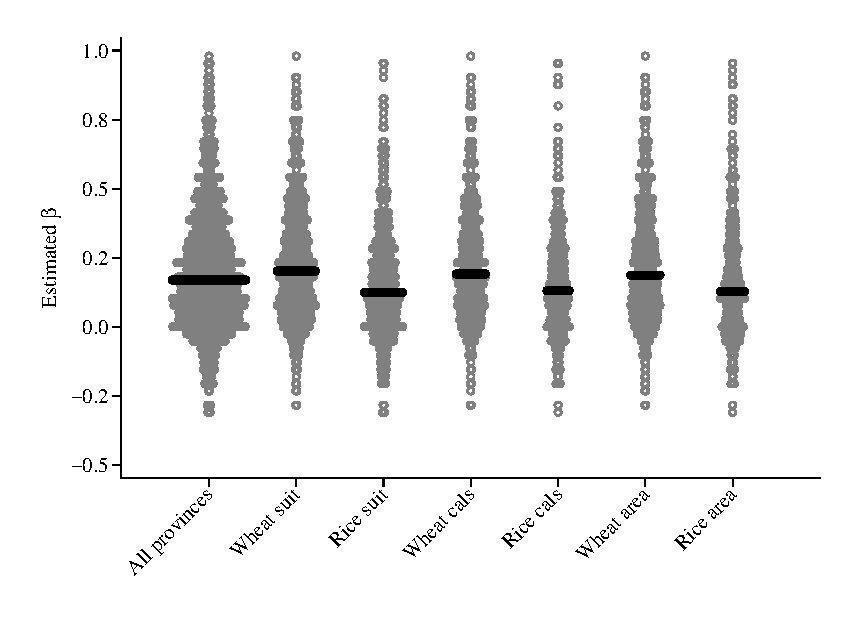
\includegraphics[width=1.0\textwidth]{fig_beta_province.eps}
\end{center}
\vspace{-.5cm}\singlespacing {\footnotesize \textbf{Notes}: Plotted are the values of $\beta_g$ estimated for each individual state in our dataset that contains 10 or more districts. The specification for these regressions is equation (\ref{EQ_regress}), and includes the controls for (log) night lights, (log) total population, and the percent urban. The value of rural labor/land for a state is total rural population of the state divided by total land area of the state.
}
\end{figure}
\clearpage


\section{Robustness Tables}
\listoftables

\clearpage
\begin{table}[!htb]
\begin{center}
\caption{Estimates of $\beta$ using individual crop productivity terms}
\label{TAB_indcrop}
{\footnotesize
\begin{tabularx}{\textwidth}{lXXXXXXX}
\midrule
\multicolumn{8}{l}{Panel A: Using only temperate districts defined by crop suitability} \\ \\
\multicolumn{8}{c}{Dependent variable is $A_{isg}$ measured by:} \\ \\
 & CSI & Barley & Buckwheat & Oats & Rye & W. Pot. & Wheat \\
 & (1) & (2) & (3) & (4) & (5) & (6) & (7) \\
\midrule
Log rural density   &       0.228&       0.225&       0.218&       0.222&       0.212&       0.233&       0.227\\
                    &     (0.021)&     (0.019)&     (0.023)&     (0.027)&     (0.021)&     (0.029)&     (0.019)\\
\midrule
p-value $\beta=0$   &       0.000&       0.000&       0.000&       0.000&       0.000&       0.000&       0.000\\
Countries           &          91&          91&          69&          68&          68&          91&          91\\
Observations        &       10661&       10628&        9699&        9834&        9804&       10597&       10631\\
Adjusted R-square   &        0.24&        0.21&        0.18&        0.23&        0.21&        0.23&        0.22\\

\midrule
\\
\multicolumn{8}{l}{Panel B: Using only tropical districts defined by crop suitability} \\ \\
\multicolumn{8}{c}{Dependent variable is $A_{isg}$ measured by:} \\ \\
 & CSI & Cassava & Cowpea & P. Millet & Sw. Pot. & Wet Rice & Yams \\
 & (1) & (2) & (3) & (4) & (5) & (6) & (7) \\
\midrule
Log rural density   &       0.132&       0.137&       0.137&       0.145&       0.136&       0.134&       0.133\\
                    &     (0.018)&     (0.022)&     (0.019)&     (0.018)&     (0.019)&     (0.028)&     (0.020)\\
\midrule
p-value $\beta=0$   &       0.000&       0.000&       0.000&       0.000&       0.000&       0.000&       0.000\\
Countries           &          81&          76&          80&          79&          79&          75&          79\\
Observations        &        9088&        8843&        9074&        8265&        9066&        8448&        9020\\
Adjusted R-square   &        0.12&        0.10&        0.11&        0.07&        0.11&        0.05&        0.10\\

\midrule
\end{tabularx}
}
\end{center}
\vspace{-.5cm}\singlespacing {\footnotesize The panels differ in the districts included in each regression. In Panel A, only districts that are suitable for temperate agriculture are inclueded (based on the criteria we outline in the paper based on GAEZ suitability measures). In Panel B, on tropical districts are included. The columns differ by the variable used to measure $A_{isg}$, inherent agricultural productivity. Column (1) uses the CSI index from Galor and Ozak (2016), as in our baseline results. Columns (2)-(7) use the raw potential yield (in tonnes) of the crop, from the GAEZ, for the crop specified. Additional controls are as in our basline results, and include province fixed effects. Conley standard errors, adjusted for spatial auto-correlation, are shown in parentheses. 
}
\end{table}

\clearpage


\begin{table}[!htb]
\begin{center}
\caption{Estimates of Land Elasticity, $\beta$, by K{\"o}ppen-Geiger Zone, 2000CE}
\label{TAB_beta_kg}
{\footnotesize
\begin{tabularx}{\textwidth}{lXXXXXX}
\midrule
\multicolumn{7}{l}{Dependent Variable in all panels: Log caloric yield ($A_{isg}$)} \\ \\
\multicolumn{7}{l}{Panel A: Climate Zones} \\
 & Equatorial & Arid & Temperate & Snow  &     &   \\
 & (1) & (2) & (3) & (4) &  & \\
\midrule
Log rural density   &       0.111&       0.154&       0.169&       0.230\\
                    &     (0.015)&     (0.026)&     (0.017)&     (0.026)\\
\midrule
p-value $\beta=0$   &       0.000&       0.000&       0.000&       0.000\\
p-value $\beta=\beta^{Equa}$&            &       0.151&       0.007&       0.000\\
Countries           &          79&          56&          94&          40\\
Observations        &       11461&        2822&       13717&        6327\\
Adjusted R-square   &        0.11&        0.10&        0.15&        0.19\\

\midrule
\\
\multicolumn{7}{l}{Panel B: Precipitation Zones} \\
& Fully     & Dry         & Dry        &              &            & \\
& Humid & Summer & Winter & Monsoon & Desert & Steppe \\
 & (1) & (2) & (3) & (4) & (5) & (6) \\
\midrule
Log labor/land ratio ($\beta_g$)&       0.240&       0.215&       0.124&       0.125&       0.130&       0.147\\
                    &     (0.044)&     (0.063)&     (0.022)&     (0.039)&     (0.072)&     (0.029)\\
\midrule
p-value $\beta=0$   &       0.000&       0.001&       0.000&       0.001&       0.072&       0.000\\
p-value $\beta=\beta_{Humid}$&            &       0.739&       0.020&       0.043&       0.190&       0.072\\
Countries           &          78&          37&          67&          32&          20&          49\\
Observations        &       13545&        2373&        7695&        1267&         146&        1735\\
R-square (ex. FE)   &        0.17&        0.17&        0.15&        0.17&        0.17&        0.16\\

\midrule
\\
\multicolumn{7}{l}{Panel C: Temperature Zones} \\
    & Hot        & Warm        & Cool       & Hot      & Cold     &  \\
    & Summer & Summer & Summer & Arid & Arid &   \\
 & (1) & (2) & (3) & (4) & (5) &  \\    
\midrule
Log labor/land ratio ($\beta_g$)&       0.142&       0.226&       0.207&       0.140&       0.190\\
                    &     (0.021)&     (0.053)&     (0.076)&     (0.035)&     (0.046)\\
\midrule
p-value $\beta=0$   &       0.000&       0.000&       0.007&       0.000&       0.000\\
p-value $\beta=\beta_{Humid}$&            &       0.065&       0.405&       0.969&       0.254\\
Countries           &          57&          82&          18&          42&          25\\
Observations        &        8101&        9003&         340&        1230&         956\\
R-square (ex. FE)   &        0.20&        0.23&        0.20&        0.17&        0.21\\

\midrule
\end{tabularx}
}
\end{center}
\vspace{-.5cm}\singlespacing {\footnotesize \textbf{Notes}: Conley standard errors, adjusted for spatial auto-correlation with a cutoff distance of 500km, are shown in parentheses. All regressions include province fixed effects, a constant, and controls for the district urbanization rate and log density of district nighttime lights. The coefficient estimate on rural population density indicates the value of $\beta_g$. Inclusion of districts is based on whether they have more than 50\% of their land area in the given K{\"o}ppen-Geiger zone. See text for details.
}
\end{table}
\clearpage
\begin{table}[!htb]
\begin{center}
\caption{Country-level aggregate land elasticity estimates, from grid-cell level}
\label{TAB_beta_country}
{\tiny
\begin{tabularx}{\textwidth}{lXlXlXlX}
\midrule
Country & $\beta$ & Country & $\beta$ & Country & $\beta$ & Country & $\beta$ \\
\midrule
Afghanistan &     0.234 & Denmark &     0.285 & Libya &     0.176 & Saint Vincent a &     0.126 \\
Akrotiri and Dh &     0.285 & Djibouti &     0.126 & Liechtenstein &     0.285 & Samoa &     0.127 \\
Albania &     0.226 & Dominica &     0.126 & Lithuania &     0.285 & San Marino &     0.167 \\
Algeria &     0.196 & Dominican Repub &     0.142 & Luxembourg &     0.285 & Saudi Arabia &     0.162 \\
American Samoa &     0.126 & Ecuador &     0.167 & Macao &     0.167 & Senegal &     0.126 \\
Andorra &     0.285 & Egypt &     0.166 & Macedonia &     0.237 & Serbia &     0.237 \\
Angola &     0.165 & El Salvador &     0.127 & Madagascar &     0.154 & Sierra Leone &     0.126 \\
Anguilla &     0.126 & Equatorial Guin &     0.127 & Malawi &     0.163 & Singapore &     0.126 \\
Antigua and Bar &     0.126 & Eritrea &     0.139 & Malaysia &     0.126 & Sint Maarten &     0.126 \\
Argentina &     0.195 & Estonia &     0.285 & Mali &     0.129 & Slovakia &     0.282 \\
Armenia &     0.283 & Ethiopia &     0.160 & Malta &     0.167 & Slovenia &     0.280 \\
Aruba &     0.126 & Fiji &     0.129 & Martinique &     0.126 & Solomon Islands &     0.126 \\
Australia &     0.189 & Finland &     0.285 & Mauritania &     0.128 & Somalia &     0.128 \\
Austria &     0.285 & France &     0.266 & Mauritius &     0.149 & South Africa &     0.198 \\
Azerbaijan &     0.214 & French Guiana &     0.126 & Mayotte &     0.126 & South Korea &     0.209 \\
Bahamas &     0.134 & Gabon &     0.126 & Mexico &     0.177 & South Sudan &     0.126 \\
Bahrain &     0.167 & Gambia &     0.126 & Moldova &     0.262 & Spain &     0.224 \\
Bangladesh &     0.164 & Georgia &     0.232 & Mongolia &     0.285 & Sri Lanka &     0.128 \\
Barbados &     0.126 & Germany &     0.285 & Montenegro &     0.248 & Sudan &     0.129 \\
Belarus &     0.285 & Ghana &     0.126 & Montserrat &     0.126 & Suriname &     0.126 \\
Belgium &     0.285 & Greece &     0.218 & Morocco &     0.204 & Swaziland &     0.176 \\
Belize &     0.131 & Grenada &     0.126 & Mozambique &     0.148 & Sweden &     0.285 \\
Benin &     0.126 & Guadeloupe &     0.126 & Myanmar &     0.153 & Switzerland &     0.284 \\
Bhutan &     0.232 & Guatemala &     0.160 & Namibia &     0.177 & Syria &     0.255 \\
Bolivia &     0.152 & Guernsey &     0.285 & Nepal &     0.191 & São Tomé and  &     0.129 \\
Bonaire, Sint E &     0.126 & Guinea &     0.127 & Netherlands &     0.285 & Taiwan &     0.183 \\
Bosnia and Herz &     0.259 & Guinea-Bissau &     0.126 & New Caledonia &     0.153 & Tajikistan &     0.223 \\
Botswana &     0.150 & Guyana &     0.126 & New Zealand &     0.285 & Tanzania &     0.150 \\
Brazil &     0.135 & Haiti &     0.132 & Nicaragua &     0.128 & Thailand &     0.132 \\
British Virgin  &     0.126 & Honduras &     0.138 & Niger &     0.126 & Timor-Leste &     0.129 \\
Brunei &     0.126 & Hong Kong &     0.167 & Nigeria &     0.126 & Togo &     0.126 \\
Bulgaria &     0.245 & Hungary &     0.244 & North Korea &     0.274 & Tonga &     0.126 \\
Burkina Faso &     0.126 & India &     0.151 & Northern Cyprus &     0.246 & Trinidad and To &     0.126 \\
Burundi &     0.186 & Indonesia &     0.129 & Norway &     0.285 & Tunisia &     0.171 \\
Cambodia &     0.126 & Iran &     0.248 & Oman &     0.128 & Turkey &     0.239 \\
Cameroon &     0.129 & Iraq &     0.210 & Pakistan &     0.188 & Turkmenistan &     0.273 \\
Canada &     0.284 & Ireland &     0.285 & Palestina &     0.224 & Turks and Caico &     0.126 \\
Cape Verde &     0.134 & Isle of Man &     0.285 & Panama &     0.129 & Uganda &     0.137 \\
Caspian Sea &     0.259 & Israel &     0.237 & Papua New Guine &     0.136 & Ukraine &     0.283 \\
Cayman Islands &     0.126 & Italy &     0.199 & Paraguay &     0.159 & United Arab Emi &     0.184 \\
Central African &     0.126 & Jamaica &     0.126 & Peru &     0.159 & United Kingdom &     0.285 \\
Chad &     0.126 & Japan &     0.203 & Philippines &     0.129 & United States &     0.225 \\
Chile &     0.279 & Jersey &     0.285 & Poland &     0.285 & Uruguay &     0.167 \\
China &     0.217 & Jordan &     0.264 & Portugal &     0.191 & Uzbekistan &     0.272 \\
Colombia &     0.141 & Kazakhstan &     0.284 & Puerto Rico &     0.128 & Vanuatu &     0.129 \\
Comoros &     0.132 & Kenya &     0.146 & Qatar &     0.167 & Venezuela &     0.130 \\
Costa Rica &     0.140 & Kosovo &     0.271 & Republic of Con &     0.126 & Vietnam &     0.149 \\
Croatia &     0.227 & Kuwait &     0.167 & Reunion &     0.193 & Virgin Islands, &     0.126 \\
Cuba &     0.126 & Kyrgyzstan &     0.283 & Romania &     0.249 & Western Sahara &     0.139 \\
Curaçao &     0.126 & Laos &     0.153 & Russia &     0.283 & Yemen &     0.126 \\
Cyprus &     0.272 & Latvia &     0.285 & Rwanda &     0.244 & Zambia &     0.166 \\
Czech Republic &     0.285 & Lebanon &     0.234 & Saint Kitts and &     0.126 & Zimbabwe &     0.164 \\
Côte d'Ivoire &     0.126 & Lesotho &     0.270 & Saint Lucia &     0.126 & Åland &     0.285 \\
Democratic Repu &     0.133 & Liberia &     0.126 & Saint Pierre an &     0.285 &  &         . \\

\midrule
\end{tabularx}
}
\end{center}
\vspace{-.5cm}\singlespacing {\footnotesize \textbf{Notes}: This table reports the aggregated value of the land elasticity, $\beta$, for each country. The aggregate value is a weighted average of the value for tropical pixels (0.088), temperate pixels (0.239), and ``both'' pixels (0.131) that can grow both tropical and temperate crops. The weights in the average are the maximum calories that can be produced in a pixel relative to the maximum calories that can be produced by all pixels in the country. 
}
\end{table}


\clearpage
\begin{table}[!htb]
\begin{center}
\caption{Estimates of $\beta$ for cash crops}
\label{TAB_indcrop}
{\footnotesize
\begin{tabularx}{\textwidth}{lXXXXXX}
\midrule
\multicolumn{7}{c}{Dependent variable is $A_{isg}$ measured for:} \\ \\
 & Banana & Coffee & Cotton & Sugarcane & Tea & Tobacco \\
 & (1) & (2) & (3) & (4) & (5) & (6)  \\
\midrule
Log rural density   &       0.197&       0.152&       0.178&       0.139&       0.267&       0.152\\
                    &     (0.046)&     (0.034)&     (0.032)&     (0.028)&     (0.064)&     (0.038)\\
\midrule
p-value $\beta_g=0$ &       0.000&       0.000&       0.000&       0.000&       0.000&       0.000\\
Countries           &          26&          24&          35&          26&          38&          54\\
Observations        &         598&         643&        1078&         745&         615&        1088\\
Harv. perc. min     &        0.23&        0.50&        0.46&        0.67&        0.06&        0.25\\

\midrule
\end{tabularx}
}
\end{center}
\vspace{-.5cm}\singlespacing {\footnotesize Each column is the result of a regression of the (log) productivity of the specified cash crop on the labor/land ratio. Districts included in each column are those where the percent of total harvested area in the specified crop is above the 99th percentile for the percent across all districts in our dataset. State fixed effects are included, as our our standard controls for (log) night lights, (log) total population, and the urban percent. Standard errors clustered at the state level are reported.
}
\end{table}

\clearpage
\begin{table}[!htb]
\begin{center}
\caption{Estimates of $\beta$ for terrain classes}
\label{TAB_indcrop}
{\footnotesize
\begin{tabularx}{\textwidth}{lXXXXXX}
\midrule
\multicolumn{7}{c}{Dependent variable is $A^{GAEZ}_{isg}$:} \\ \\
 & \multicolumn{6}{c}{Excluding districts with terrain index:} \\
 & \multicolumn{2}{c}{Below 1st ptile:} & \multicolumn{2}{c}{Below 5th ptile:} & \multicolumn{2}{c}{Below 25th ptile:} \\ \cmidrule(lr){2-3} \cmidrule(lr){4-5} \cmidrule(lr){6-7}
 & Temperate & Tropical & Temperate & Tropical & Temperate & Tropical \\
 & (1) & (2) & (3) & (4) & (5) & (6)  \\
\midrule
Log labor/land ratio ($\beta_g$)&       0.233&       0.089&       0.213&       0.088&       0.179&       0.078\\
                    &     (0.047)&     (0.020)&     (0.044)&     (0.020)&     (0.031)&     (0.018)\\
\midrule
p-value $\beta_g=0$ &       0.000&       0.000&       0.000&       0.000&       0.000&       0.000\\
p-value $\beta_g=\beta_{Temp}$&            &       0.004&            &       0.009&            &       0.005\\
Countries           &          84&          76&          80&          76&          71&          73\\
Observations        &        9284&        7224&        8822&        7151&        6977&        6377\\
R-square (ex. FE)   &        0.24&        0.20&        0.23&        0.19&        0.23&        0.18\\

\midrule
\end{tabularx}
}
\end{center}
\vspace{-.5cm}\singlespacing {\footnotesize Sets of regressions differ by exclusion of districts based on their terrain index (GAEZ). A lower terrain index indicates a more rugged terrain, so the regressions are exluding rugged areas, and including only flatter districts. State fixed effects are included, as our our standard controls for (log) night lights, (log) total population, and the urban percent. Standard errors clustered at the state level are reported.
}
\end{table}

\end{document}